\documentclass[11pt]{article}
\title{\textbf{Neuronale Netze} \\ Zusammenfassung}
\author{Marius Bauer}
\date{\today}

\usepackage{ngerman}
\usepackage[T1]{fontenc}
\usepackage[utf8x]{inputenc}
\usepackage{graphicx}
\usepackage{enumitem}
\usepackage[left=2.5cm,right=2.5cm]{geometry}


% Mathematik
\usepackage{amsmath}
\usepackage{amsfonts}
\usepackage{amssymb}

% should be loaded last
\usepackage{hyperref}

\hypersetup {
	pdftoolbar=true, % Anzeigen der Acrobat toolbar oder nicht
	pdfmenubar=true, % Anzeigen des Acrobat menu oder nicht
	pdftitle={Neuronale Netze Zusammenfassung},
	pdfsubject={Neuronale Netze},
	pdfauthor={Marius Bauer},
	pdfkeywords={Neuronale, Netze, TDNN, Autoencoder},
	pdfcreator={texmaker},
	%linkcolor=rot, 	% Farbe der internen Verweise
	%citecolor=grün, 	% Farbe der Zitate
	%urlcolor=magenta, 	% Farbe der Links
	colorlinks=false, 	%Links sind farbig 
	%linkbordercolor=rot,	% Roter Rahmen
	%citebordercolor=grün, 	% Grüner Rahmen
	%urlbordercolor=cyan,	% Cyan farbiger Rahmen 
	pdfborderstyle={/S/U/W 1},
	%pdfborder={0 0 0} % gar keine Boxen um Links
}

% preferences
\setenumerate{noitemsep}

\begin{document}
\maketitle
\newpage
\tableofcontents
\newpage

% ################## search for TODO ################

\section{Neuronale Netze - kurzer Überblick}
\label{sset:neuronale-netze-kurzer-überblick}
\textbf{Wieso werden neuronale Netze verwendet?}
\begin{itemize}
	\item Massive parallelism.
	\item Massive constraint satisfaction for ill-defined input.
	\item Simple computing units.
	\item Many processing units, many interconnections.
	\item Uniformity (-> sensor fusion)
	\item Non-linear classifiers/ mapping (-> good performance)
	\item Learning/ adapting
	\item Brain like ??
\end{itemize}
\textbf{Wofür werden neuronale Netze verwendet?}
\begin{itemize}
	\item Classification
	\item Prediction
	\item Function Approximation
	\item Continuous Mapping
	\item Pattern Completion
	\item Coding
\end{itemize}
\textbf{Welche Kriterien müssen beim Entwurf von neuronalen Netzen beachtet werden?}
\begin{itemize}
	\item Recognition Error Rate
	\item Training Time
	\item Recognition Time
	\item Memory Requirements
	\item Training Complexity
	\item Ease of Implementation
	\item Ease of Adaptation
\end{itemize}
\textbf{Welche Parameter werden typsicherweise vom Entwerfer bestimmt?}
\begin{itemize}
	\item Net Topology
	\item Node Characteristics
	\item Learning Rule
	\item Objective Function
	\item (Initial) Weights
	\item Learning Parameters
\end{itemize}
\textbf{Wo werden neuronale Netze verwendet?}
\begin{itemize}
	\item Space Robot*
	\item Autonomous Navigation*
	\item Speech Recognition and Understanding*
	\item Natural Language
	\item Processing*
	\item Music*
	\item Gesture Recognition
	\item Lip Reading
	\item Face Recognition
	\item Household Robots
	\item Signal Processing
	\item Banking, Bond Rating
	\item Sonar
\end{itemize}
\textbf{Advanced Neural Models}
\begin{itemize}
	\item Time-Delay Neural Networks (Waibel)
	\item Recurrent Nets (Elman, Jordan, Robinson,..)
	\item Higher Order Nets
	\item Modular System Construction
	\item Adaptive Architectures
	\item Hybrid Neural/Non-Neural Architectures
	\item Deep Nets
\end{itemize}
\textbf{Welche Probleme können beim Entwurf von neuronalen Netzen auftreten?}
\begin{itemize}
	\item Local Minima
	\item Speed of Learning
	\item Architecture must be selected
	\item Choice of Feature Representation
	\item Scaling
	\item Systems, Modularity
	\item Treatment of Temporal Features and Sequences
\end{itemize}
\textbf{Eigenschaften von neuronalen Netzen:}
\begin{itemize}
	\item non-linear classifier
	\item approximate posterior probability
	\item non-parametric training
\end{itemize}
\newpage

\section{Pattern Recognition}
\label{sect:pattern-recognition}
\begin{figure}[h]
	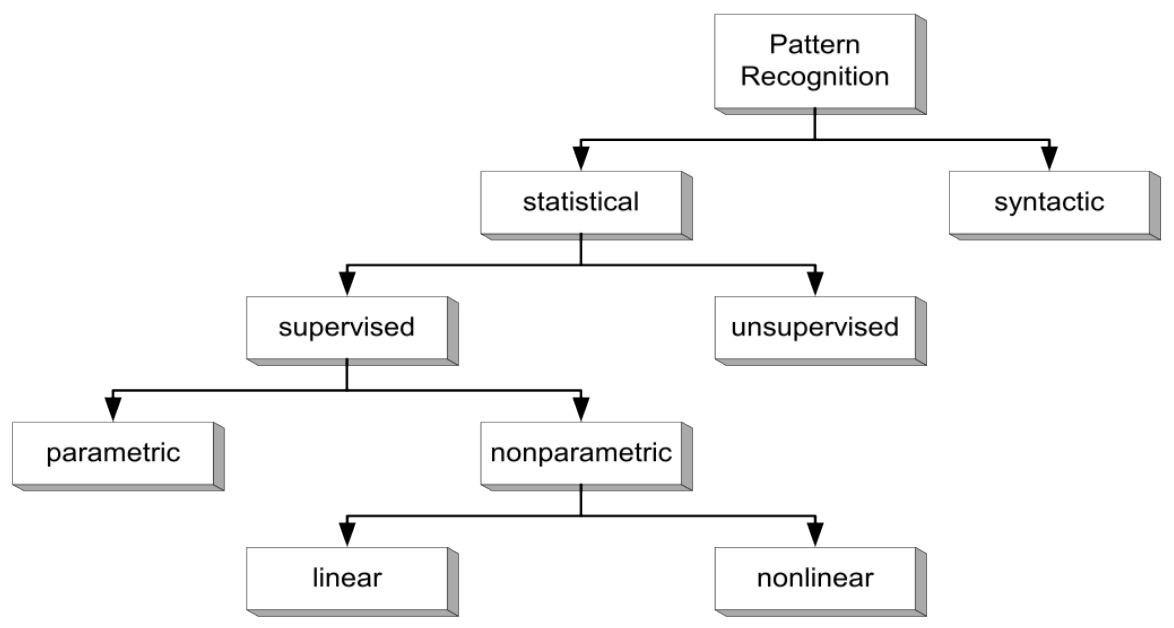
\includegraphics[scale=0.3]{pattern-recognition-partitioning}
\end{figure}

\begin{itemize}
	\item supervised:
		\begin{itemize}
			\item labels / classes of training data are known
			\item train a classifier
		\end{itemize}
	\item unsupervised:
		\begin{itemize}
			\item labels / classes are not known
			\item find the structure of the data
			\item methods: clustering, autoassociative nets
		\end{itemize}
	\item parametric:
		\begin{itemize}
			\item assume underlying probability distribution
			\item estimate the parameters
			\item eg.: Gaussian classifier
		\end{itemize}
	\item unparametric:
		\begin{itemize}
			\item doesn't assume underlaying probability distribution
			\item estimate probability of error from training data
			\item nearest neighbours, parzen window, perceptron
		\end{itemize}
\end{itemize}

\subsection{Bayes Decision Theory - Parametric}
\label{ssect:bayes-decision-theory}
\begin{align*}
P(\omega_j |x) &= \frac{p(x|\omega_j) \cdot P(\omega_j)}{p(x)} \\
p(x) &= \sum_j p(x|\omega_j) \cdot P(w_j)
\end{align*}
Since we have overlapping probability distribution false classifications occur. Simply speaking to reduce false classification always decide for the class with the highest probability (errors still can occur!).

\subsection{Classifier Discrimination Function}
\label{ssect:classfier-discrimination-function}
The \textit{classifier discrimination function} iterats over all classes and choses those which has the highest probability. In the case of the Gaussian classifier it looks as follows:
\begin{align*}
g_i &= P(\omega_i | x) \\
&= p(x | \omega_i) \cdot P(\omega_i) \\
&= \log(p(x | \omega_i)) + \log(P(\omega_i))
\end{align*}
Problems:
\begin{itemize}
	\item limited traning data
	\item limited computation
	\item class-labeling potentially costful and errorful
	\item classes or features might not be known
\end{itemize}
Parametric solution: assume that $p(x|\omega_i)$ has a parametric form. The most common representative: multivariant normal density.\\
Univariant normal density:
\[
p(x) = \frac{1}{\sqrt{2 \cdot \pi \sigma}} \cdot e^{(-\frac{1}{2} \cdot \frac{x - mu}{\sigma})^2}
\]
Multivarian normal density:
\[
p(\overleftarrow{x}) = \frac{1}{\sqrt[d]{2 \pi} \cdot \sqrt{|\Sigma|}} \cdot e^{-\frac{1}{2} \cdot \frac{(\overleftarrow{x} - \overleftarrow{\mu})^2}{\Sigma}}
\]
The following form takes effect for the classifier discrimination function:
\[
g_i(\overleftarrow{x}) = -\frac{1}{2} \cdot \frac{(\overleftarrow{x} - \overleftarrow{\mu_i})^2}{\Sigma_i} - \frac{d}{2} \cdot \log(2\pi) - \frac{1}{2} \cdot \log(|\Sigma_i|) + \log(P(\omega_i))
\]
For the Gaussian classifier we have to estimate the \textit{covariance matrix} $\Sigma_i$ and the \textit{mean vector} $\mu_i$. To estimate the parameters we can use the \textit{MLE: maximum likelihood estimation} for the univariant case.
For the multivariant case we can use:
\[
\overleftarrow{\mu} = \frac{1}{N} \cdot \Sigma_{k = 1}^{N} \overleftarrow{x_k}
\]
\[
\Sigma = \frac{1}{N} \cdot \Sigma_{k = 1}^{N} (\overleftarrow{x_k} - \overleftarrow{\mu}) \cdot (\overleftarrow{x_k} - \overleftarrow{\mu})^T
\]
\subsection{Curse of Dimensionality}
\label{ssect:curse-of-dimensionality}
The problem with the classifier design in general is that we can not say which features are the most valuable ones, are more features better and is features are useful will they be ignored? \\
However in general we can say that more features performe worse because we have limited training data and we still have to estimate the parameters (Eg. 1000 sample training data and 1000 parameters to estimate). We have to select the best feature and might have to reduce the dimensions (for example with the \textit{Principle Component Analysis (PCA)}.

\subsubsection{Principle Component Analysis (PCA)}
\label{sssect:principle-component-analysis-pca}
The idea is that single dimension are correlated and we want to remove the dimension with the least informations:
\begin{itemize}
	\item[1.] find the axis with the highest variance
	\item[2.] rotate the space along the axis
	\item[3.] not the dimensions are uncorrelated
	\item[4.] remove the dimension with the lower variance
\end{itemize}

\subsection{Non-Parametric Methods}
\label{ssect:non-parametric-methods}
\textit{Non-Parametric Methods} do not assume any distributions and try to find structures in the data itself.

\subsubsection{Parzen Window}
\label{sssect:parzen-window}
\begin{itemize}
	\item[1.] chose a window with volume $V$
	\item[2.] count the numbers of samples in that window $p(x) = \frac{\frac{k}{N}}{V}$ where $k$ are the samples in the window and $N$ is the total numbers of samples.
\end{itemize}
The hard part is to chose the window size. the thumb roule is: $V_n = \frac{1}{\sqrt{n}}$

\subsubsection{k-nearest Neighours}
\label{sssect:k-nearest-neighbours}



\newpage
\section{Recurrent Neural Networks}
\label{sect:recurrent-neural-networks}
\textit{Recurrent Neural Networks} unterscheiden sich von anderen neuronalen Netzen in dem Punkt, dass sie einen (oder mehrere) Zustände speichern und verwenden können. Dabei ist ein Zustand ein berechneter Wert des vorherigen Zeitschritts. Diese Zustände können widerrum als Input genutzt werden. Somit ist eine zeitliche Zustandsspeicherung möglich.

\subsection{Sequence Learning}
\label{ssect:sequence-learning}
Sequenzen sind überall in unserem alltäglichem Leben vertreten: z.B. bei der Sequenzierung von Töne in Sprache. Bei der Spracherkennung wird der Fokus auf Wortsequenzen gelegt. 
Bei sequence learning gibt es vier generelle Probleme:
\begin{itemize}
	\item sequence prediction: Was wird das nächste Element in der Sequenz sein?
	\item sequence generation: generieren einer Sequenz (eg. Wortsequenz)
	\item sequence recognition: Ist die Sequenz legitim?
	\item sequence decision making: ??
\end{itemize}
% properly refer to the picture
\begin{figure}[h]
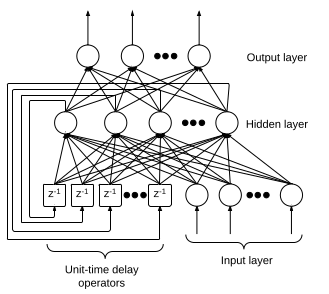
\includegraphics[scale=1.0]{rnn-example1}
\end{figure}

\subsection{Elman vs. Jordan Networks - Simple RNN}
\label{ssect:elman-vs-jordan-networks-simple-rnn}
Der Unterschied zwischen \textit{Elman} und \textit{Jordan} Netzen besteht darin, dass sie unterschiedliche Outputs zwischenspeichern und wiederverwenden. Bei Elman Netzen wird der Output des Hidden Layers als Input für den nächsten Zeitschritt verwendet. Jorden Netze auf der anderen Seite nutzen den Output des Netzes als Input für den nächsten Zeitschritt.

\subsection{Aufbau}
\label{ssect:rnn-aufbau}
% TODO: insert graphic of a rnn
\begin{itemize}
	\item Input Units $X = x_1, x_2, ..., x_n$
	\item Output Units $Y = y_1, y_2, ..., y_n$
	\item Hidden Units $H = h_1, h_2, ..., h_n$
	\item Connections between Units
\end{itemize}
Im Prinzip sehen RNN genauso aus wie NN. Jedoch sind die Verbindungen anders. Diese können nämlich zurückführen und als Input dienen. Somit lassen sich vergangene States wiederverwenden. Alternative könnte man \textit{recurrent hidden units} in den Aufbau mit aufnehmen. Diese speichern vergangene Zustände und leiten diese als Input in den darauffolgenden Zeitschritt in die entsprechenden Units.
\subsection{Training}
\label{ssect:rnn-training}
RNN werden mittels \textit{backpropagation through time} trainiert. Dies ist eine Erweiterung des ursprünglichen Backpropagation, bei der die wiederkehrenden Zustände berücksichtigt werden. Dazu wird ein RNN \textit{ausgerollt} um den zeitlichen Zusammenhang darzutellen:
\begin{figure}
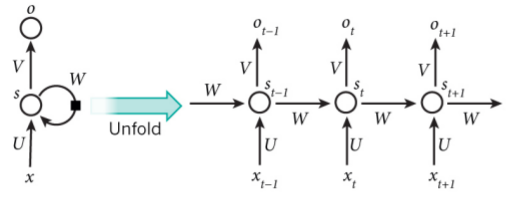
\includegraphics[scale=0.6]{unfold-example}
\end{figure}
Zu jedem Zeitpunkt nutzen wir \textit{forward pass} um die Aktivität in jedem Zeitschritt zu berechnen. Mittels \textit{backward pass} wird die Fehlerableitung zu jedem Zeitschritt berechnet.
In dem entrollten Netzwerk kommen die selben Gewichte öfters vor (shared weights), zu sehen in Bild XX. Jede Instanz eines Gewichtes muss den selben Gradienten erhalten (Einschränkung):
\begin{itemize}
	\item[1.]$w_j^{t_1} = w_j^{t_2} \Rightarrow \Delta w_j^{t_1} = \Delta w_j^{t_2}$
	\item[2.]Berechne $\frac{\partial E}{\partial w_j^{t_1}}$ und $\frac{\partial E}{\partial w_j^{t_2}}$
	\item[3.] $\Delta w_j^{t_1} = \Delta w_j^{t_2} = -\eta \left(\frac{\partial E}{\partial w_j^{t_1}} + \frac{\partial E}{\partial w_j^{t_2}}\right)$
\end{itemize}
Hierbei kann zum einen die Summe betrachtet werden, aber auch der Durchschnitt!

\subsection{Vanishing / Exploding Gradient}
\label{ssect:vanishing-exploding-gradient}


\newpage
\section{Backpropagation}
\label{sect:backpropagation}
Improve BP
\begin{itemize}
	\item Parallel Hardware
	\item Efficient Implementation
	\item Faster Gradient Descent Search
	\item Selective Choice of Patterns
	\item Efficient Architectures
\end{itemize}
\begin{figure}[h]
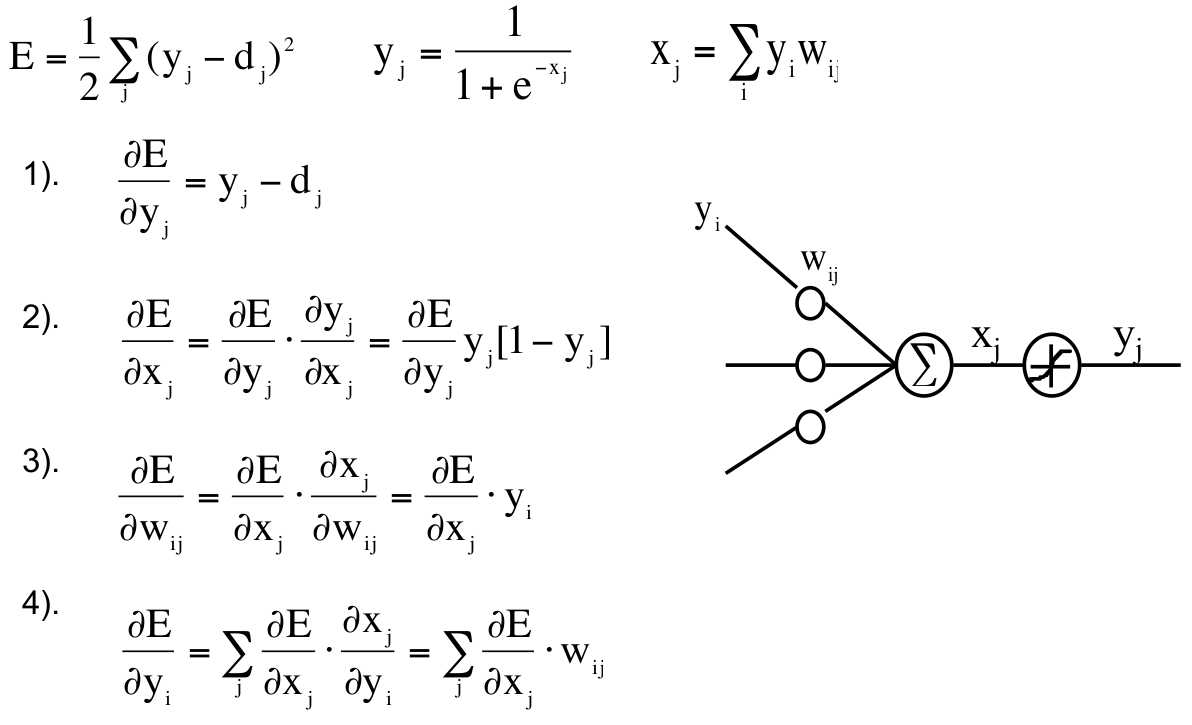
\includegraphics[scale=0.35]{bp}
\end{figure}
The weight update faces different problems: vanishing / exploding gradient, small weights update (slow learning), etc. One way to fix some of the problems is to set a \textit{step size} and \textit{momentum} to the weight update:
\[
\Delta w_{ij}(t) = - \epsilon \frac{\delta E}{\delta w_{ij}(t)} + \alpha \Delta w_{ij}(t - 1) 
\]
$\epsilon$ is the step size (or learning rate) and $\alpha$ is the momentum. The momentum says how much of the last weight update should be added to the current weight update. This will prevent slow training a little.\\[1cm]
Eine weitere Beschleunigung des Trainings erhält man indem für bestimmte Beispiel kein BP angewende wird. Hierbei muss der Fehler groß genug sein, ansonsten wird der Fehler ignoriert.\\[2cm]
Ebenso können wir die Lernrate dynamisch anpassen, um zu verhindern, dass weight updates hin und her springen.
\begin{figure}[h]
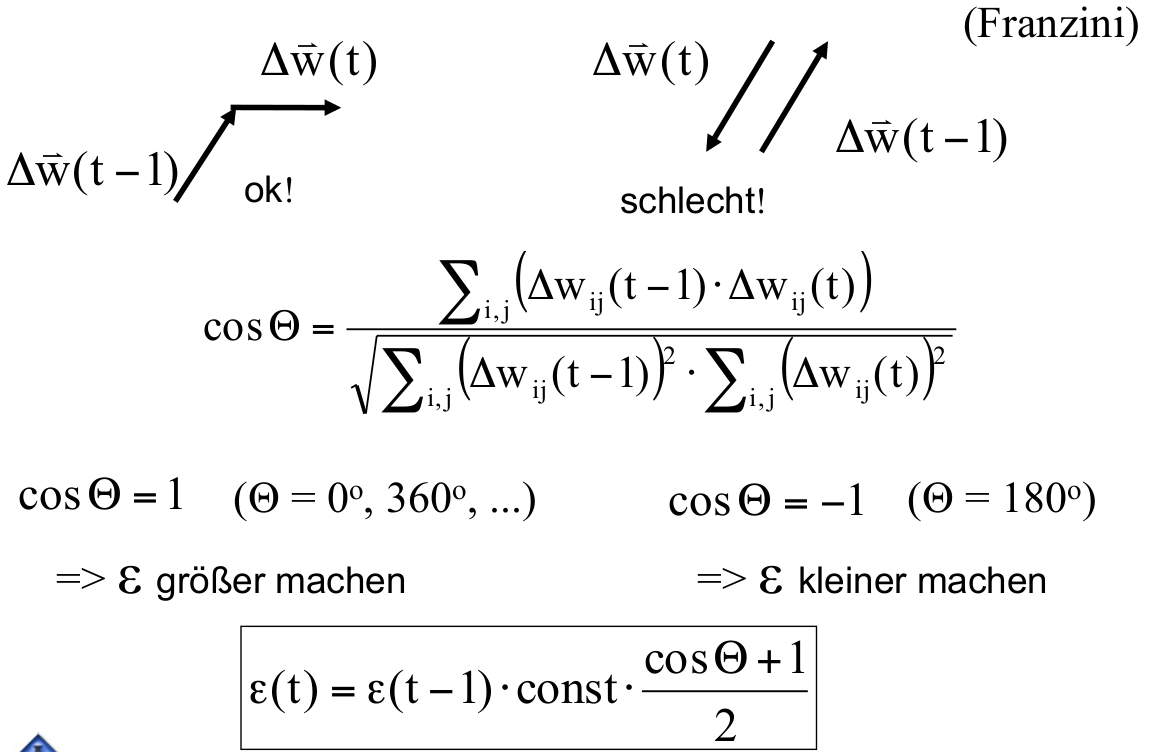
\includegraphics[scale=0.3]{dynamic-learning-rate}
\end{figure}\\[1cm]
Um ein MLP schnell trainieren zu können, kann sich der \textit{Quickprop Algorithmus} eignen:
\[
\Delta w(t) = \frac{s(t)}{s(t - 1) - s(t)} \cdot \Delta w(t-1)
\]
wobei $s(t) = \frac{\delta E}{\delta w_{ij}}(t)$. Jedoch hängt das schnelle Training nicht nur vom Lernalgorithmus ab. The initial weight should be initialist by looking at the activation function and look for the intervall with the biggest derivant.
\textbf{Generalisierung}: The generalization states how well the system will perform on the validation set.\\
Reasons:
\begin{itemize}
	\item Overfitting
	\item too much parameters or too less trainings data
	\item wrong topology
\end{itemize}
Generalization for linear Systems:
\[
\langle \epsilon_{test} \rangle = \langle \epsilon_{train} \rangle + 2 \sigma^2 \frac{p}{n}
\]
Generalization for linear Systems:
\[
\langle \epsilon_{test} \rangle = \langle \epsilon_{train}(\lambda) \rangle + 2 \sigma^2_{eff} \frac{p_{eff}(\lambda)}{n}
\]

Methods to better generalization:
\begin{itemize}
	\item reduce network complexity (weight decay, weight elimination, optimal brain damage, optimal brain surgeon): prevent overfitting
	\item stepwis increase of size of network (cascade correlation, meiosis network, automativ structure optimization): incresae size of network so it can learn
\end{itemize}

\subsection{Regularization}
\label{ssect:regularization}
Regularization is used to prevent overfitting.

\subsubsection{Weight Elimination}
\textit{Weight Elimination} is added to the error to punish the network for large weights ($\lambda$: 0.0001...0.001):
\[
E = MSE + \lambda \sum_{i,j} \frac{w_{i,j}^2}{1 + w_{i,j}^2}
\]
\begin{itemize}
	\item - slow learnin
	\item - worse performance on trainingsdata
	\item + better generalization
\end{itemize}

\subsubsection{Optimal Brain Damage}
\label{sssect:optimal-brain-damage}
Idea: remove certrain connection of the network to reduce the complexity of the network and prevent overfitting. Easy: remove connections with very small $|w_{i,j}|$. Better: remove thos connections which influence the error the smallest (unimportant weights). Therefore calculate:
\[
\frac{\delta E}{\delta w_{ij}^2}
\]
\subsubsection{Cascade Correlation}
\label{sssect:cascade-correlation}
\begin{figure}[h]
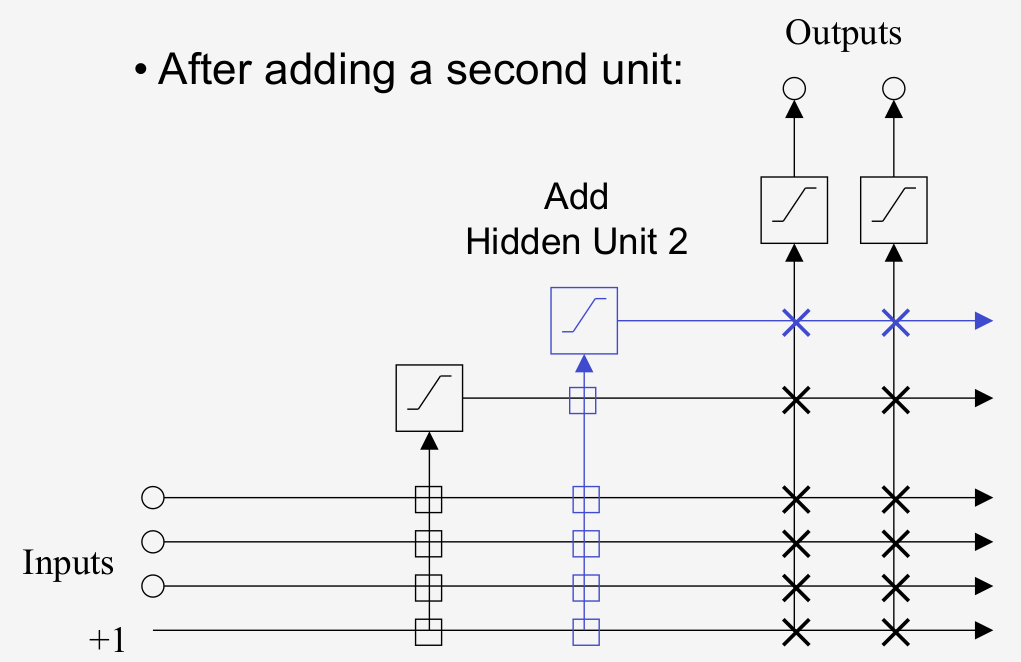
\includegraphics[scale=0.4]{cascade-correlation}
\end{figure}
\begin{itemize}
	\item can create deep networks without a drastic slowdown
	\item amount hidden unis does not need to be estimated empirisch 
	\item each time step only one layer of connections is trained
	\item learns very fast
	\item incremental learning
\end{itemize}

\subsubsection{Meiosis Network}
\label{sssect:meiosis-network}
Idea: adding of hidden unis depends on the ''uncertainty'' of the network. The mean and varianz is learned.
\[
w_{ij}^{*} = \mu(w_{ij}) + \sigma(w_{ij}) \phi(0, 1)
\]
Start with one hidden unit and split unit if
\[
\frac{\sum_i \sigma_{ij}}{\sum_i \mu_{ij}} > 1.0 \: and \: \frac{\sum_k \sigma_{ik}}{\sum_k \mu_{ik}} > 1.0
\]
\section{Speech}
\label{sect:speech}
Die Sprachproduktion beim menschlichen Körper besteht aus drei Teilen: 1. dem supraglottale Sprachtrakt, 2. dem kehlkopf und 3. dem subglottalem System (teil davon ist die Lunge). Die Lunge und der Kehlkopf werden dabei über motorische Bewegung angeregt. Genauer gesagt, die Lunge stellt die Luft bereit, welche vom Kehlkopf benötigt wird um angeregt zu werden. Die Lunge und der Kehlkopf zusammen sorgen somit für die \textit{Anregung}.
Je nach ''Form'' des Vokaltrakts (Rachen-, Mund- und Nasenraum) kommt es durch die Anregung zu einer anderen \textit{Artikulation}. Dabei werden Töne erzeugt und ''ausgegeben''. Aneinander gereihte Töne ergeben dadurch Sprache.
Die verschiedenen Töne produzieren verschiedene Spektrale. Für bestimmte Laute bzw. Vokale lassen sich typische Muster im Spektralbereich finden und somit die Vokale unterscheiden.

\subsection{Speech Recognition}
\label{ssect:speech-recognition}
\begin{figure}[h]
\centering
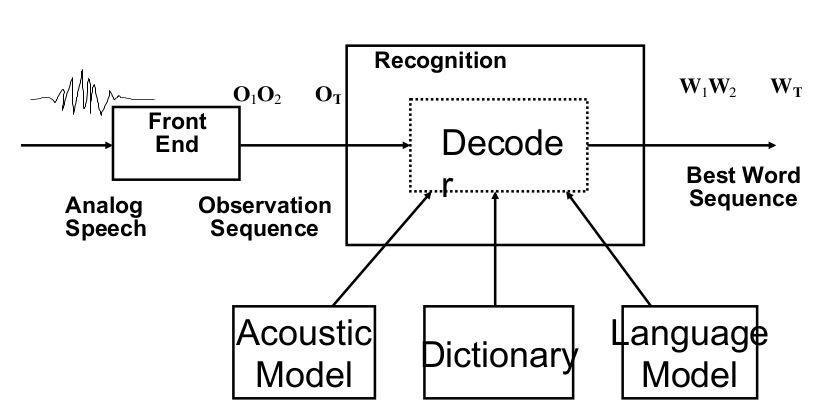
\includegraphics[scale=0.45]{komponenten-speech-recognition}
\label{graph:komponenten-speech-recognition}
\caption{Komponenten eines Sprach Erkenners}
\end{figure}
Auf dem obigen Bild sind die einzelnen Komponenten eines Sprach Erkenners zu sehen. Links kommts das \textit{analoge Signal} in das Front End rein und wird digitalisiert. Dazu wird es mittels Fouriertransformation in den Spektralbereich umgewandelt. Aus dem Frontend kommt die \textit{observation sequence} heraus und wird an den \textit{Decoder} weitergegeben. Im Decoder passiert die eigentliche Sprach Erkennung. Dazu wird ein \textit{acoustic model}, ein \textit{dictionary} und ein \textit{language model} verwendet. Die einzelnen Komponenten werden wir uns später noch genauer anschauen. Der Decoder gibt am Ende die \textit{best word sequence} aus.
Das Ziel des Sprach Erkenners ist es aus einer gegebenen akkustichen Daten $A = a_1, a_2, ..., a_k$ die Wortsequenz $W = w_1, w_2, ..., w_n$ zu finden, welche die Wahrscheinlichkeit $P(W|A)$ maximiert. Dazu brauchen wir die \textit{Bayes Regel}:
\[
P(W|A) = \frac{P(A|W) \cdot P(W)}{P(A)}
\]
P(W|A) ist das \textit{acoustic model}, P(W) ist das \textit{language model} und P(A) ist konstant für einen ganzen Satz.

\subsection{Acoustic Model}
\label{ssect:acoustic-model}

\subsubsection{Hidden Markov Model}
\label{sssect:hidden-markov-model}
Elements:
\begin{itemize}
	\item states: $S = \langle S_0, S_1, ..., S_N\rangle$
	\item transition probabilities: $P(q_t = S_i | q_{t-1} = S_j) = aji$
	\item emission probabilities: $P(y_t = O_k | q_t = S_j) = b_j(k)$
\end{itemize}
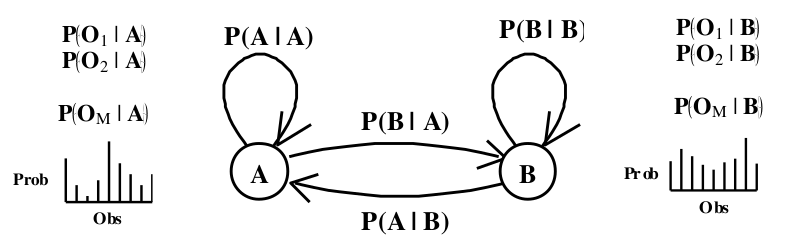
\includegraphics[scale=0.45]{hhm-example}
In der Spracherkennung spiegeln die States die phonetischen Zustände wieder (genauer gesagt besteht jedes Phonem aus drei Zuständen: beginning, middle und end). Der Decoder sucht hierbei den besten Pfad zwischen den Modellen und der Sprache.
Um die Emissionswahrscheinlichkeit zu approximieren können neben HMMs alternative Methoden verwendet werden:
\begin{itemize}
	\item Mixture of Gaussians Networks
	\item Neural Networks
	\item Hierarchies of Neural Networks
\end{itemize}

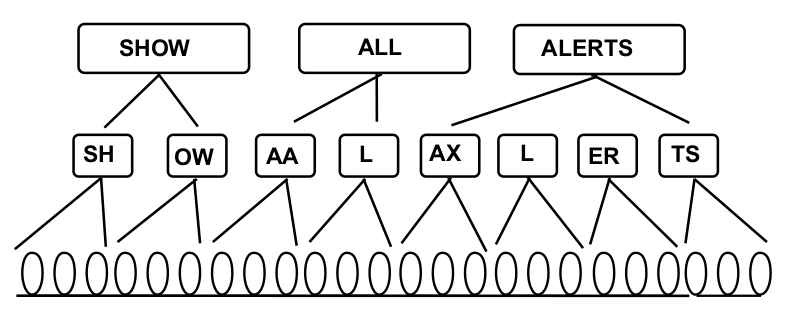
\includegraphics[scale=0.5]{alignment-phoneme-sprache}
Die Wörter werden zerlegt in Phoneme und die Phoneme in Zustände.

\subsubsection{Time Delay Neural Network (TDNN)}
\label{sssect:TDNN}
Ein \textit{time delay neural netwrok} ist eine spezielle Art von neuronalem Netz, welches \textit{time invariant} ist. Es besteht aus einem Input Layer, mehreren Hidden Layers und einem Output Layer.
Als Eingabe dient eine Matrix welche \textit{mel-scaled} ist. Die x-Achse spiegelt die Zeit wider, die y-Achse die Frequenz. Der erste Hidden Layer erhält als Eingabe ein 16 x 3 Ausschnitt der Eingabe, jeweils verschoben in der x-Richtung. Somit überlappen sich die Eingaben für den ersten Hidden Layer. Im Hidden Layer wird ebenfalls ein Fenster drüber gelegt und einem weiteren Hidden Layer als Input gegeben. Im Output Layer wird auf einzelne Buchstaben gemappt. Das bedeutet ein TDNN kann ein Muster in einem Signal finden egal wo es sich befindet. Alles was wir wissen ist, dass es darin vorkommt.
Im letzten Hidden Layer werden horizontal die Aktivierungen der Neuronen angeschaut und daraus bestimmt, welches Phonem vorgekommen ist. Der letze Hidden Layer wird auch als \textit{phoneme layer bezeichnet}. Jedoch bezieht sich das TDNN in unserem Fall auf einzelne Phoneme, jedoch werden Wörter aus mehreren Phonemen gebildet. Siehe dazu \ref{sssect:MS-TDNN}.
TDNN sind \textit{convolutional networks} mit einer festen Größe. Dies ist beim Übergang zwischen den Schichten zu sehen. Convolutional neuronale Netze werden in der Bildverarbeitung verwendet. Hierbei ist es so, dass z.B. Straßenschilder aufgenommen, aber nicht immer an der selben Stelle im Bild sind.\\
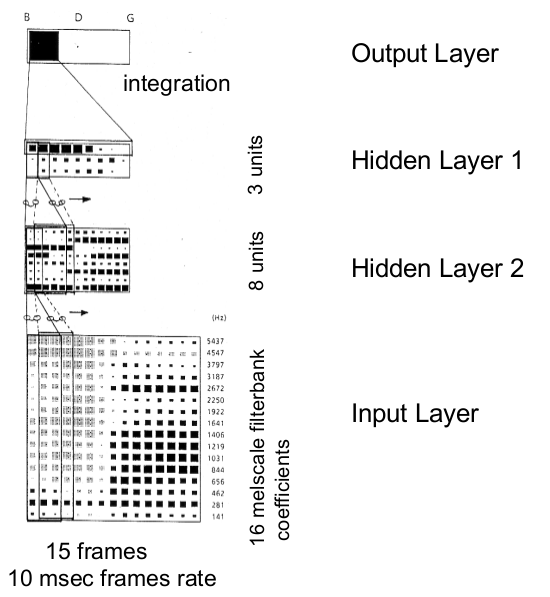
\includegraphics[scale=0.5]{tdnn}
Eine Erweiterung der TDNN stellen die \textit{frequency shifting TDNN (FSTDNN)} dar. Diese Netze sind shift invaraint in zwei Dimensionen. Das bedeute nicht nur Zeitinvariant sondern auf Frequenzinvariant. Normalerweise wird ein Netz auf eine Person trainiert und die Fehlerrate steigt, sobald eine andere Person das Netz benutzt. Die Frequenzinvarianz sorgt dafür, dass Männer, Frauen oder Kinder das selbe Nezt benutzen können und die Fehlerrate verändert sich nur gering. Dies nennt sich auch \textit{Multi-Speaker Phoneme Recognition}.
Darüber hinaus gibt es noch das Problem des Echo / der Verhallung. Wenn kein Mikrofon direkt am Mund getragen wird, wird das Signal verrauscht / verschmiert. Die Verhallung ist immer unterschiedlich und man kann kein Netz für jeden Raum bauen. Bei der Verhallung wird das ursprüngliche, gesprochene Signal mit dem Echo gefaltet. Neuronale Netze können diese Verhallung lernen und rausfiltern.
\subsection{Word Model}
\label{ssect:word-model}
Bisher haben wir nur die Erkennung von Phoneme behandelt. Diese müssen nun zu ganzen Wörtern zusammengebaut werden. Eine Idee wäre ein neuronales Netz für ein betimmtes Vokabular zu trainieren. Jedoch ist das Unsinn, da ein neues Wort bedeutet, dass man Beispiele sammeln muss und das Netz neu trainieren muss.

Problems:
\begin{itemize}
	\item Time Alignment: the same word might be spoken faster / slower
	\item Endpoint Detection: where does one word end?
	\item Large Dictionaries (Training Data, Time)
\end{itemize}

\subsubsection{Time Alignment}
\label{sssect:time-varying-patterns}
Hierbei geht es darum, dass verschiedene Sprecher unterschiedlich schnell/langsam sprechen. Irgendwie muss beim Lernen einen zeitlichen Zusammenhang herausgearbeitet werden. \\ \\
Beim \textit{Linear Sequence Alignment} wird das Referenzsignal und das unbekannte Signal linear aneinander angepasst (Stauchen / Strecken). Problem hierbei ist, dass der Mensch in der Regel nicht linear schnell redet. Wir benötigen ein \textbf{non-linear alignment}.\\ \\
Eine Lösung ist das \textit{time warping} (auch dynamic programming genannt?!?). Hierbei wird eine Verbindung zwichen zwei Sequenzen $x$ und $y$ gesucht. Die Achsen repräsentieren die Sequenzen, welche Vektoren sind, desen Einträge gut oder schlecht aufeinander passen.
Sind die Signale aufeinander abgestimmt, kann mittels des \textit{Viterbi-Algorithmus} die passende Sequenz $Q$ gefunden werden, welche $P(O, Q| \lambda)$ maximiert.

\subsubsection{Multi-State-TDNN}
\label{sssect:MS-TDNN}
Ein MS-TDNN ist eine Erweiterung des TDNN auf Wortebene. Um ein Wort zu erkennen muss eine bestimmt Sequenz von Phonemen auftretten. Im DTW-Layer(dynamic time warping) wird die Verbindung der Phoneme vorgenommen und im Output Layer lese ich das entsprechende Wort ab. Das bedeutet aber wiederum, dass ich für jedes einzelne Wort ein Output Neuron brauche. Das ist bei großen Wörterbüchern unpraktisch. Jedoch ist das nicht so schlimm, da wir auf dem Wortlevel Trainieren können. \\
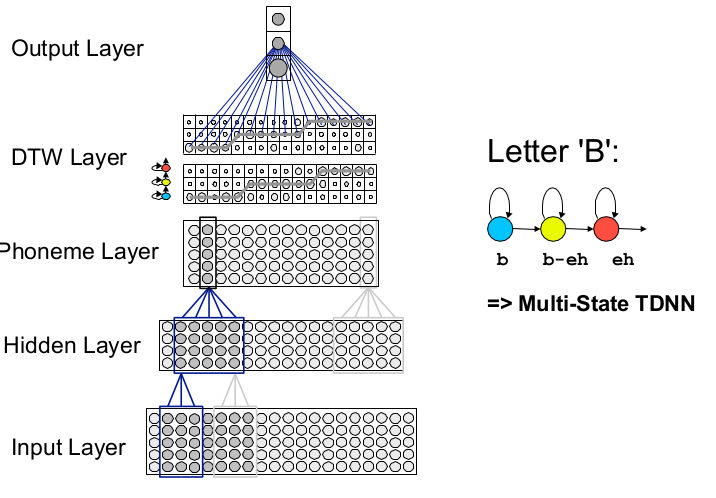
\includegraphics[scale=0.5]{MS-TDNN1}

Ich versuche die Distanz zwischen dem richtigen Wort und dem besten, falschem Wort zu maximieren. Das heißt wir optimieren die phonetische Sequenz und nicht die Wörter an sich.
Im MS-TDNN befindet sich ein Decoder. Das Alinieren der Zustände und der Feature, welche das neuronale Netz über die Zeit gelernt hat, läuft wie ein HMM mit dynamik time warping oder mit Viterbi Decoding. Der Unterschie dzu den Hypbriden, welche danach dran kommen, ist, dass das es sich hierbei um hidden Features handelt.

\subsubsection{NN-HMM Hybride}
Die Idee ist, dass ein neuronales Netz gebaut wird, welches die Phoneme erkennt. Wenn der Output statisch interpretiert werden kann, wird ein HMM Decoder obendrüber gebaut, der für das Alignment und die Integration der Wörter zuständig ist.
Die Wahrscheinlichkeit, welche wir als Output des NN bekommen, ist nicht die richige. Um die richige Wahrscheinlichkeit zu erhalten, müssen wir die Bayes Regel umformulieren. Wir wollen P(A|W) haben aber P(W|A).\\
Die (log)Wortwahrscheinlichkeit besteht aus der Summe der (log)Output Activations entlang des besten Pfades (bestimmt mit DTW oder Viterbi).

Kontextabhängige Phonemmodelle (a in Kontext von P etc.)

\subsubsection{Viterbi-Algorithmus}
\label{sssect:viterbi-algorithmus}
Der Viterbi Algorithmus sucht das beste Alignment zwischen allen phonetischen Sequenzen, die vorkommen können und der gesprochenen Sprache.
\subsubsection{Forward-Algorithmus}
\label{sssect:forward-algorithmus}

\subsubsection{Backward-Algorithmus}
\label{sssect:backward-algorithmus}

\newpage
\section{Learning Vector Quantization}
\label{sect:learning-vector-quantization}
Der initiale Ansatz ist \textit{vector quantization}, welcher als erstes besprochen wird. Die Weiterentwicklung des vector quantization ist \textit{learning vector quantization}, welche danach behandelt wird.

\subsection{Vector Quantization}
\label{ssect:vector-quantization}
Die Idee hinter vector quantization ist, dass der \textit{data space} mit einer kleinen Anzahl an \textit{prototype vectors} $U = u_1, u_2, ..., u_k$ beschrieben wird. Jeder prototype vector repräsentiert eine Klasse ($k$ Klassen). Dazu muss jeder Input Vektor $X = x_1, x_2, ..., x_m$ einem der Vektoren in $U$ zugewiesen werden. Die prototype vectors $U$ sind in einem \textit{codebook} zusammengefasst. Vector Quantization ist unsupervised.

\subsubsection{Applications}
\label{sssect:vq-application}
\begin{itemize}
	\item multimedia compression (storage and transmission)
	\item dimensionality reduction
	\item classification
\end{itemize}

\subsubsection{Training}
\label{ssect:vq-training}
Beim Trainieren werden die Input Vektoren mittels einem geeignetem Distanzmaß $d$ und einem Clustering Algorithmus unterteilt. Daraus ergeben sich die Anzahl an Klassen und somit auch direkt die Anzahl an Codebuch Einträgen. Die Vektoren im Codebuch sind die \textit{centroids} der einzelnen Regionen.
Bei der eigentlichen Klassifikation (Encoding) wird für einen Input Vektor die Distanz zu den Codebuch Einträgen berechnet und bei der minimalen Entfernung der Index des prototype vectors gemerkt (bzw. übermittelt).
Beim Decoding wird anhand des Index der jeweilige prototype vector ausgewählt und repräsentiert somit den Input Vektor. Der Fehler hierbei ist das Distanzmaß des Input Vektors und des prototype vectors.
\begin{figure}[h]
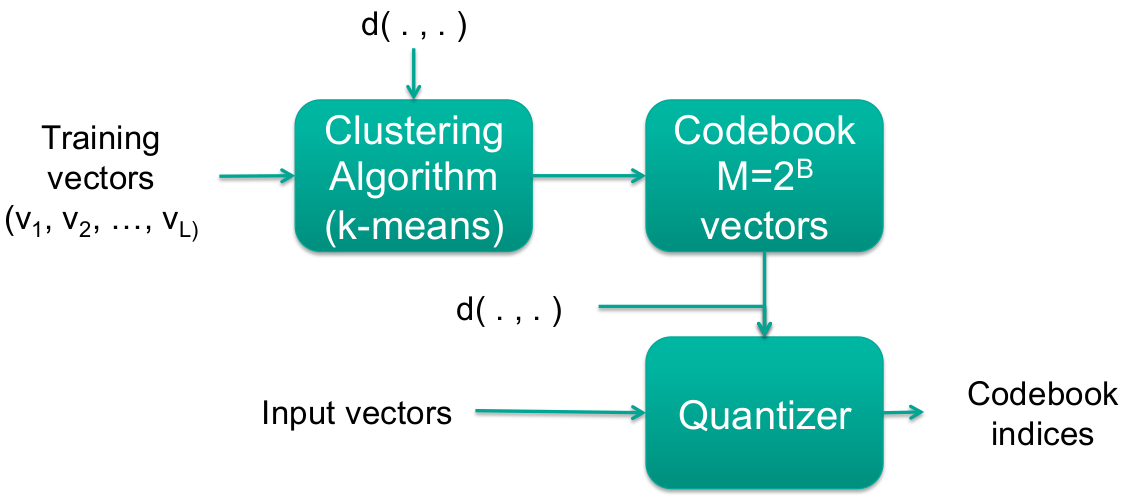
\includegraphics[scale=0.3]{vector-quantization-training}
\end{figure}

\subsection{Learning Vector Quantization}
\label{ssect:learning-vector-quantization}
Da wir nun über Labels verfügen (also wissen in welche Klasse der Input Vektor gehört), lassen sich nun Wahtscheinlichkeitsverteilungen nutzen:
\begin{itemize}
	\item $P(S_k)$: a prior Wahrscheinlichkeit der Klasse $S_k$
	\item $p(x|x \in S_k) $: bedingte Wahrscheinlichkeitsdichte 
	\item discriminant functions: $\delta_k(x) = p(x|x \in S_k) P(S_k)$
	\item rate of misclassification minimized if: $\delta_c(x) = max_k\{\delta_k(x)\}$
\end{itemize}
Prinzipiell weisen wir mehrere prototype vectors den einzelnen Klasse zu. Ein Input Vector erhält die selbe Klasse wie der prototype vector, an dem der Input Vektor am nähsten ist. Da wir nun aber mehrere prototype vectors je Klasse haben, müssen wir entscheiden, welcher der \textit{winning codebook entry} ($c$ ist der Index) ist. Die einzelnen Algorithmen unterscheiden sich in dieser Wahl:
\subsubsection{LVQ1}
\label{sssect:vq-lvq1}
$c = argmin_i\{||x - m_i||\}$: Index des prototype vectors\\
Learning rules:
\begin{itemize}
	\item $m_c(t + 1) = m_c(t) + \alpha(t)[x(t) - m_c(t)]$: $x$ und $m_c$ selbe Klasse
	\item $m_c(t + 1) = m_c(t) - \alpha(t)[x(t) - m_c(t)]$: $x$ und $m_c$ unterschiedliche Klasse
	\item $m_c(t + 1) = m_i(t)$: für $i \neq c$
\end{itemize}

\subsubsection{LVQ2}
\label{sssect:vq-lvq2}
Die Klassifizierung ist die selbe wie bei LVQ1. Das updaten ist anders:
\begin{itemize}
	\item $m_i$ und $m_j$ sind die nähsten Nachbarn von $x$ und werden simulaten geupdated.
	\item $x$ muss in ein ''window'' um $m_i$ und $m_j$ fallen.
	\item $d_i$ und $d_j$ sind die Distanzen (z.B. euklidien) zwischen $x$ und $m_i$ und $m_j$
	\item $min \left(\frac{d_i}{d_j}, \frac{d_j}{d_i}\right) > s$ where $s = \frac{1 - w}{1 + w}$ (recommended window: 0.2 to 0.3)
\end{itemize}


Ergänzungen:
$m_i$ ist der Gewinner (falsche klasse)
$m_j$ zweiter gewinner, richtige klasse -> dann updaten
$\alpha$ die Lernrate wird kleiner und kleiner

\subsubsection{LVQ2.1}
\label{sssect:vq-lvq2.1}


\subsubsection{LVQ3}
\label{sssect:vq-lvq3}



Ergänzen:
- die Frage ist welches k das korrekte ist. Zur Not kann man die Distortion betrachten und ein anderen k wählen +-
- $delta_k$ = wkeit das x zu $s_k$ gehört
- stopping rule -> fehler kleine genug oder anzahl iteration erreicht
\subsubsection{OLVQ}
\label{sssect:vq-olvq}
\section{Self-Organizing-Maps}
\label{sect:self-organizing-maps}


\subsection{Principles Of Self-Oragnized-Learning}
\label{ssect:principles-of-self-organized-learning}


\subsubsection{Principle 1: Self-Amplification}
\label{sssect:principle1-self-amplification}


\subsubsection{Principle 2: Competition}
\label{sssect:principle2:competition}


\subsubsection{Principle 3: Cooperation}
\label{sssect:principle3:cooperation}


\subsubsection{Principle 4: Structural Information}
\label{sssect:principle4:structural-information}


\subsubsection{Hebbian Learning}
\label{sssect:hebbian-learning}


\subsection{Self-Organizing-Maps}
\label{ssect:self-organizing-maps}


SOM
	theory
	structure
	learning
	properties
		VQ
	kernel SOM
	applications
\section{Reinfocement Learning}
\label{sect:reinforcement-learning}
\begin{itemize}
	\item agent can act
	\item actions change the agent's future state
	\item scalar rewards for success
	\item (sequential decision making
\end{itemize}
\textit{Select actions to maximize the future reward}.\\
Examples of Reinforcement Learning:
\begin{itemize}
	\item Fly stunt maneuver in a	 helicopter
	\item Defeat the world champion at backgammon	
	\item Manage an investment portfolio
	\item Control a power station
	\item Make a humanoid robot walk
	\item Play many different Atari games better than humans	
\end{itemize}
\begin{figure}[h]
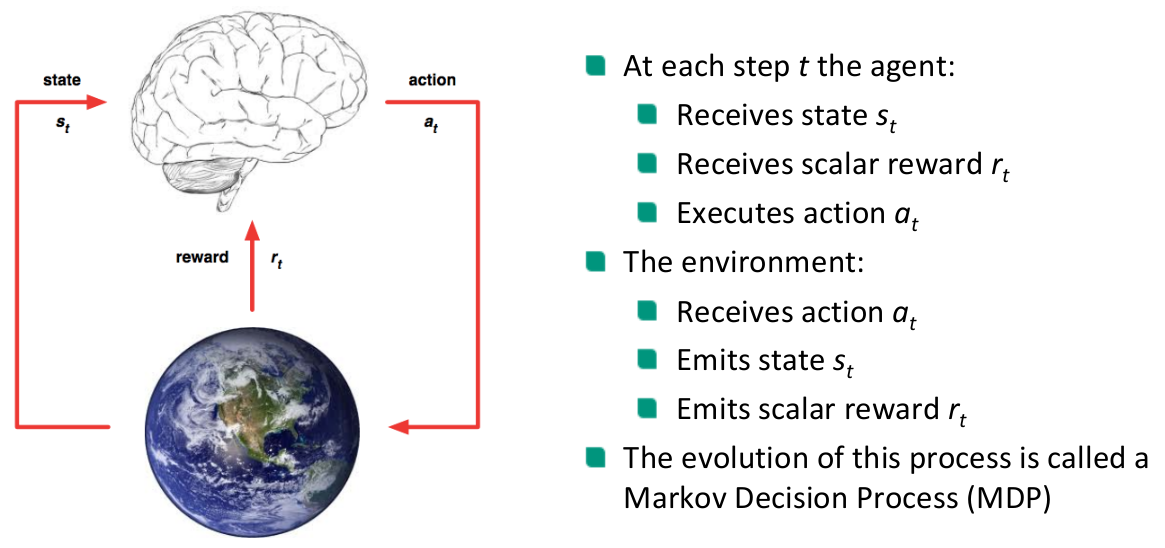
\includegraphics[scale=0.4]{agent-and-environment}
\end{figure}
\textbf{Policy} $a = \pi(s)$: probabilty distribution of actions given a state\\
\textbf{Value function} $Q^{\pi}(s, a)$: expected total reward from state $s$ and action $a$ under policy $\pi$
\[
Q^{\pi}(s, a) = \mathbb{E}[r_{t + 1} + \gamma r_{t + 2} + \gamma^2 r_{t + 2} + \gamma^3 r_{t + 3} + ... | s, a]
\]
\textbf{Policy-based RL}: search directly for the optimal policy $\pi$ (achieving maximum future reward)\\
\textbf{Value-based RL}: estimate optimal value function $Q^*(s, a)$ (maximum value achievable under any policy)\\
To train these networks we use \textit{Monte Carlo methods} to learn from experience.
\textbf{Policy-based Reinforcement Learning}: parameterize the policy (for example with a neural network) and based on the cumulative rewards, update the policy. We need to get the gradient of the rewards with respect to the policy:
\begin{itemize}
	\item Policy Gradients algorithm
	\item Online: update after episode
	\item Offline: update while in episodes
\end{itemize}
\begin{figure}[h]
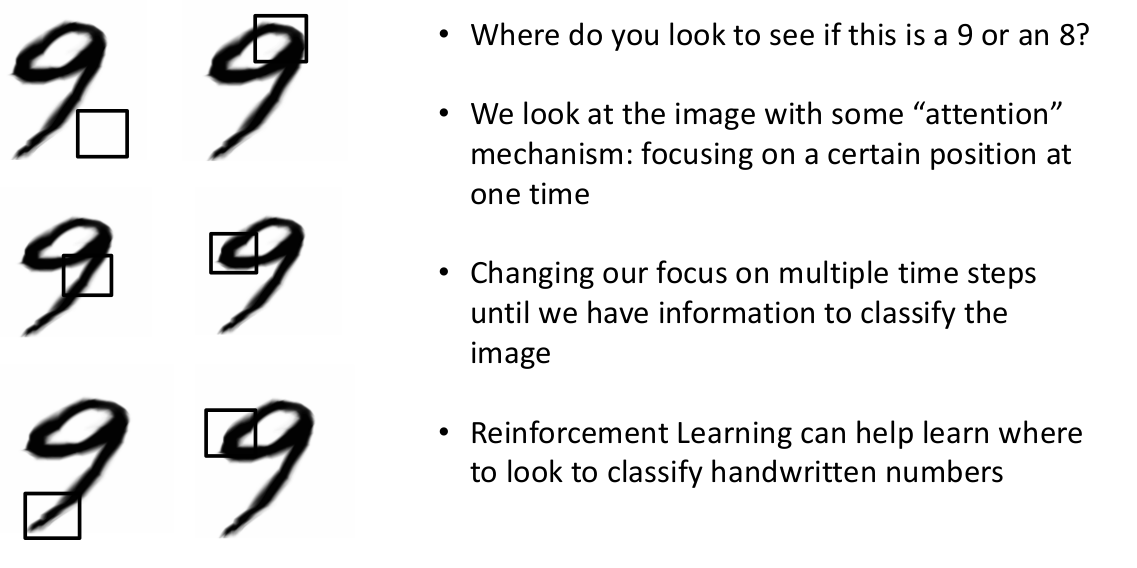
\includegraphics[scale=0.4]{policy-gradients-with-neural-networks}
\end{figure}
For the image shown we can use a RNN to determine what our current state is given the last state. RL for where should we look next, given our current states.
\begin{figure}[h]
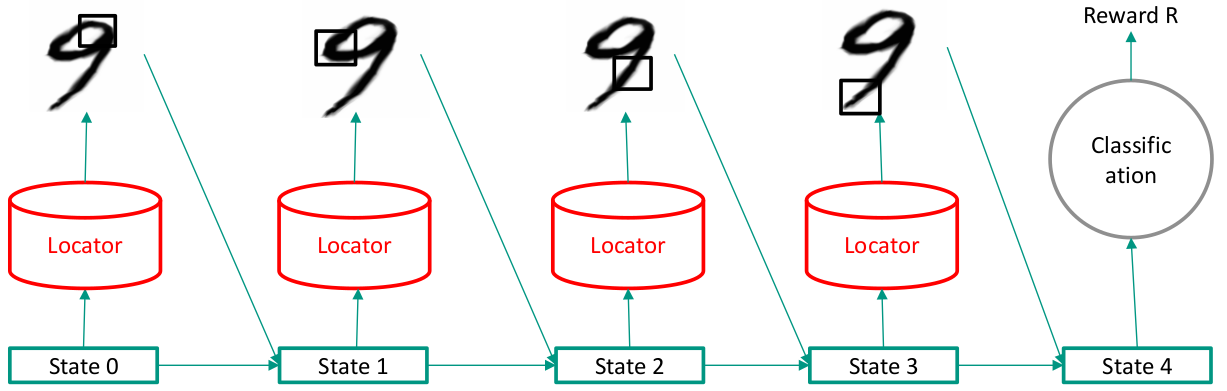
\includegraphics[scale=0.4]{RL-rrn-rl}
\end{figure} \\
RL gives use an reward on which we can calculate the backward pass (reward represents the gradient).
\begin{figure}[h]
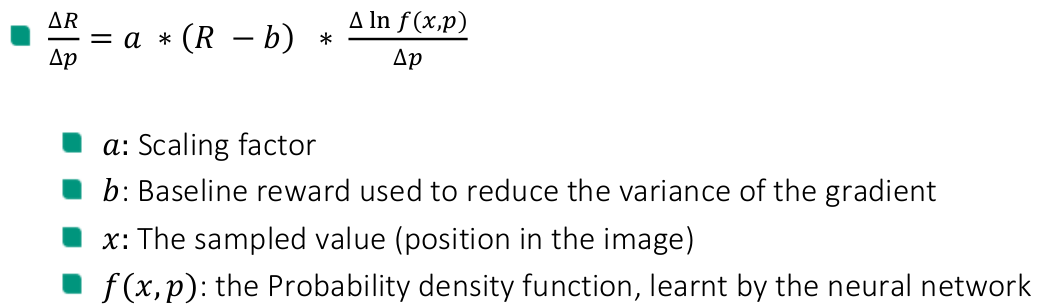
\includegraphics[scale=0.4]{policy-gradient-with-neural-networks}
\end{figure}\\[2cm]

\subsection{Bellman Equation}
\label{ssect:bellman-equation}
\[
Q^{\pi}(s, a) = \mathbb{E}[r_{t + 1} + \gamma r_{t + 2} + \gamma^2 r_{t + 2} + \gamma^3 r_{t + 3} + ... | s, a]
\]
Recursively:
\[
Q^{\pi}(s, a) = \mathbb{E}_{s^{'}}[r_{t + 1} + \gamma Q^{\pi}(s^{'}, a^{'})| s, a]
\]
Optimal value function:
\[
Q^{*}(s, a) = \mathbb{E}_{s^{'}}[r_{t + 1} + \gamma Q^{\pi}(s^{'}, a^{'})| s, a]
\]
Value iteration solve the Ballman Equation:
\[
Q_{i + 1}(s, a) = \mathbb{E}_{s^{'}}[r_{t + 1} + \gamma Q_i(s^{'}, a^{'})| s, a]
\]


\newpage
\section{Deep Learning in Computer Vision}
\label{sect:deep-learning-in-computer-vison}
class: was sieht man im bild?
local: was sieht man und wo? (bounding boxes)
detection: local + 
segmentation: trivial

low/mid/high - level: wie viele pixel betrachtet werden

rezeptives Feld: beim pooling wird rausgezoomt, der betrachtete Bildbereich wird vergrößert.
- pooling fördert die betrachung von lokalen zusammenhängen (die ohne nvlt nicht zu erkennen sind)
- überlappung fördert invarianz
 stationarity (translational invariance): 
 	V19F17: wenn das bild durchgeschoben wird, wird denoch die selbe wkeit detektiert (aber in unterschiedlichen Neuronen)
CNN: convolutional layer, sub sampling layer, fully connected MLP
multiple convolution

Image caption with attention

Calculate Parameters of NNs
\section{Neural Network Applications in Machine Translation}
\label{sect:neural-network-applications-in-machine-translation}
NLP vs MT

\newpage
\section{Speaker Independence}
\label{sect:speaker-independence}
Normal TDNNs are time invariance. However men, women and children differ in \textit{frequency}. Men normally have a darker voice than women and children. Therefore we have to compensate this invariance.


Observations on TDNNs
\begin{itemize}
	\item TDNNs develope linguistically plausible features in the hidden units
	\item TDNNS developed alternate internal representations that can link quite different acoustic realizations to the same higher level concept (because of multilayer arrangement)
	\item hidden units fire synchrony because they operate independent of precise time alignment or segmentation (time invariant)
	\item small network output may not be useful in complex task (but the internal abstractions may be valuable)
	\item complex concepts -> use stages with different knowledge
	\item new learning strategies should be build in existing knowledge
\end{itemize}
Model invariance
\begin{itemize}
	\item frequency shift, tilt, compression
\end{itemize}
Variability
\begin{itemize}
	\item adaption
		\begin{itemize}
			\item slow adaption -> modify weights
			\item fast adaption -> pretrained specific submodels
		\end{itemize}
	\item normalization
		\begin{itemize}
			\item environment: to the room
			\item speaker: mapping new speaker to standard speaker (with standard sentences)
		\end{itemize}
\end{itemize}
Combine \textbf{two standard TDNNs} to one (overall better classification): one with MSE and the other with CFM. Those combination yields the correct classification.\\
Even better than two TDNNs: \textbf{three TDNNS}! The third TDNN uses CE.

\subsection{Frequency Invariance}
\label{ssect:frequency-invariance}
\textit{Convolutional Acoustic Models}:
\begin{itemize}
	\item parameter sharing across spectrum and time -> exploit 2D structure of features
	\item upper layer fully connected
	\item pooling gives more robustness and less overfitting
\end{itemize}

\subsection{Multi-Speaker Reference Model}
\label{ssect:multi-speaker-reference-model}
Idea: A speaker-specific reference model is composed from several well trained reference models:
\begin{figure}[h]
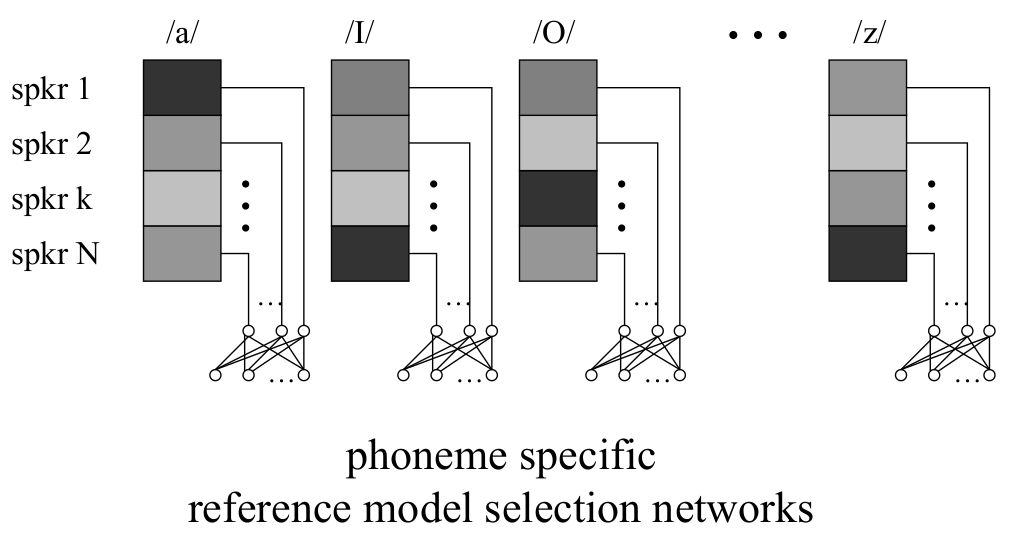
\includegraphics[scale=0.4]{phoneme-specific-reference-model-selection-networks}
\end{figure}\\
Meta-Pi-Net:
\begin{figure}[h]
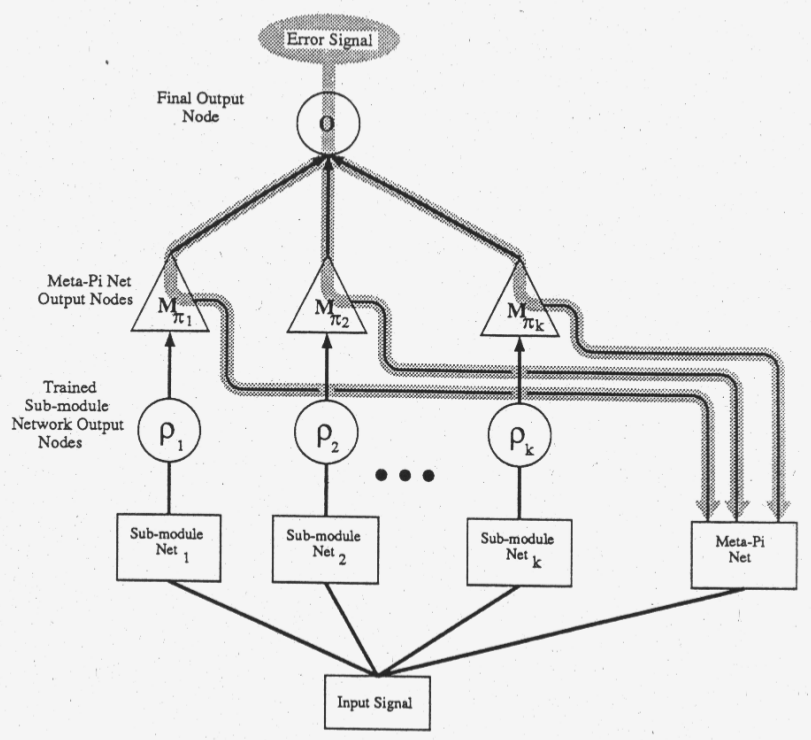
\includegraphics[scale=0.4]{meta-pi-model}
\end{figure}\\
A seperate neural net \textit{Meta-Pi-Net} controls the activation / deactivation of the single nets. The whole net is a combination of one net per speaker. In general we look which speaker net is closest to the input (which nets classifies the best). The Meta-Pi-Net produces weights for each net which control how much each net is taking into account for the classification.\\
It is not important that the correct speaker is chosing. Sometimes a combination of two or more speaker might fit better to the input. The actual correct speaker net might not be even taking into account (results in a mixture of the other nets).\\[1cm]

\textbf{Speaker Normalization}: we have speaker dependent nets. Now when we use those nets to classifier what another speaker says (no dependent net for this speaker!) the error rate is 41.9\%. With 40 text-dependent training sentences the error rate is reduced to 6.8\%.

\textbf{i-vectors}: identity vectors (i-vectors) describe the speaker-characteristic offset to an universal background model. Those i-vecotrs are used to train a recognition system.\\[1cm]

\textit{Speaker Adaptive Training of DNN}:
\begin{itemize}
	\item[1.] train initial DNN with (and keep it fixed)
		\begin{itemize}
			\item SI features: fbank
			\item SA features: Feature space Maximum Likelihood Linear Regression (fMLLR)
		\end{itemize} 
	\item[2.] Train an i-vector NN
		\begin{itemize}
			\item inputs: i-vectors
			\item outputs: linear shift to the original feature vectors
			\item added features become speaker-normalized
		\end{itemize}
	\item[3.] update the DNN in the new feature space, i-vector NN fixed -> yields SAT-DNN
\end{itemize}

\subsection{Cross-Language DNNs}
\label{ssect:cross-language-dnns}
\textit{Multilingual Bottleneck Features}:
\begin{itemize}
	\item Humans can only produce a finite amount of different sounds
	\item Subset of sounds is used in individual languages
	\item Some sounds are used in different languages
	\item Share data of the same sounds from different languages
	\item Extract more robust features using data with more variability
\end{itemize}
\begin{figure}[h]
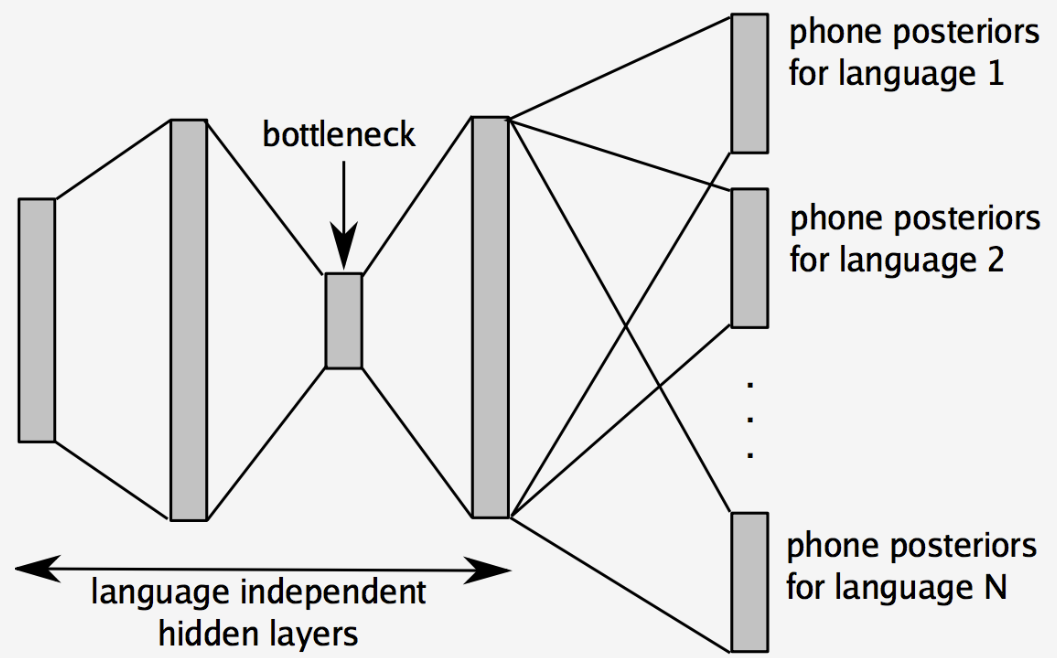
\includegraphics[scale=0.4]{multilingual-bottleneck-features}
\end{figure}
Cross-Language DNNs with Language-Universal Feature Extractors:
\begin{figure}[h]
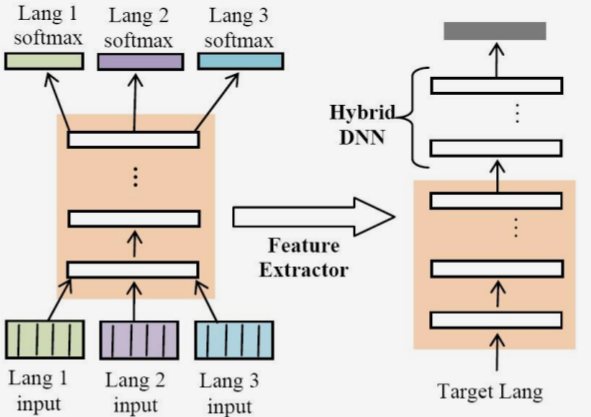
\includegraphics[scale=0.4]{DNNs-LUFE}
\end{figure}\\
DNNs can be trained on mutltiple languages. The hidden layers (\textit{language-universal feature extractor}) are used in other DNNs.

\newpage
\section{Hand Writing}
\label{sect:hand-writing}

\newpage
\section{Natural Language Processing}
\label{sect:natural-language-processing}
NN applications in NLP
\begin{itemize}
	\item Classification/Sequence labeling problems
	\item Language Modeling and Word Embeddings
	\item Sentence Modeling
	\item Machine Translation
	\item Dialog Systems
\end{itemize}
Tasks Of NLP:
\begin{itemize}
	\item Part-Of-Speech: label each word
	\item Chunking: label segments of a sentence (noun or verb phrase)
	\item Named Entity Recognition: label atomic elements (person, locatin)
	\item Semantic Role Labeling: label elements of a sentence with a semantic role 
\end{itemize}
\textbf{Window of n-gram}: $k$ words before, $k$ words after currentl 
considering word: $n= 2*k + 1$
\textbf{1-of-N coding(one-hot)}: a vocabulary-size-dimensional vector, 1 in the index of the word, 0 otherwise.

\subsection{Language Model}
\label{ssect:language-model}
Model how fluent a sentence is. Given sentence S, calculate P(S). Given incomplete sentence H, calculate P(wordX | H).Probability of the next word given a history (MLE):
\[
P(w_i|H) = P(w_i | w_1 ... w_{i-1}) = \frac{count(w_1 ... w_i)}{count(w_1 ... w_{i-1})}
\]
Conventional n-gram approach (only n previous words):
\[
P(w_i|H) \approx P(w_i | w_{i-n+1} ... w_{i-1}) = \frac{count(w_1 ... w_i)}{count(w_{i-n+1} ... w_{i-1})}
\]
Probability of the whole sentence S:
\[
P(S) = P(w_1 ... w_N) \approx \Pi_{i=1}^N P(w_i | w_{i-n+1} ... w_{i-1})
\]
\begin{figure}[h]
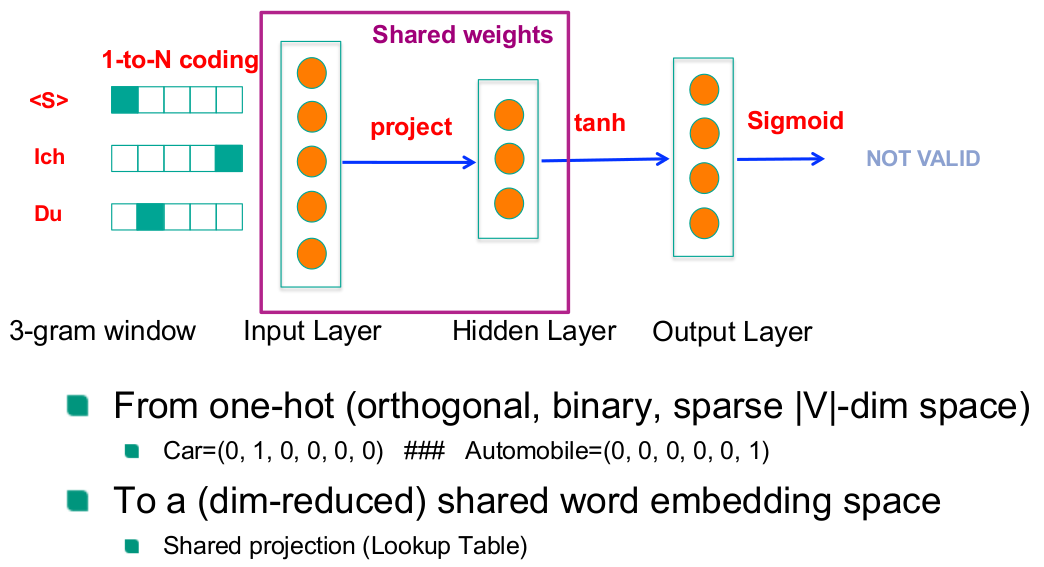
\includegraphics[scale=0.4]{word-embeddings}
\end{figure}
\subsubsection{Word Embeddings}
\label{sssect:word-embeddings}
Spatial distance corresponds to word similarity: we(car) close to we(automobile).\\
Vector operations can be used to combine word meanings: we(king)-we(queen) ~ we(man)-we(woman)

\subsubsection{Word2Vec}
needed??

\subsection{Sentence Modeling}
\label{ssect:sentence-modeling}
Representation of word sequences: Need fixed-length representation vectors for variable-length sequences.\\
Approaches:
\begin{itemize}
	\item Simple aggregation: Sum/Average/Max?
	\item Recurrent architectures: One word vector at a time step
	\item Recursive NN: Compositions using syntax parsed tree
	\item Time-Delay NN or Convolutional NN
\end{itemize}
Convolutional:\\
input sequence: $\mathbf{s} \in \mathbf{R}^s$\\
Filter vector: $\mathbf{m} \in \mathbf{R}^m$ (??????)\\
Take the dot product from $\mathbf{m}$ with each m-gram in $\mathbf{s}$ to obtain a sequence $\mathbf{c_j}$:
\[
\mathbf{c_j} = \mathbf{m}^T \cdot \mathbf{s}_{j-m+1:j}
\]
After convolution step we have a matrix $\mathbf{c_j}$ (sequence of vectors) but still be a variable-length sequence (on $s$): $\mathbf{c}_j \in \mathbf{R}^{m x s}$\\
Max Pooling: Take the max value of each row in $\mathbf{c_j}$ . Now we have a fixed-length vector (on $m$).\\
Exactly the same as Time-Delay Neural Networks (TDNN)

\subsubsection{Dynamic k-max Convolutional NN}
\label{sssect:dcnn}
\begin{figure}[h]
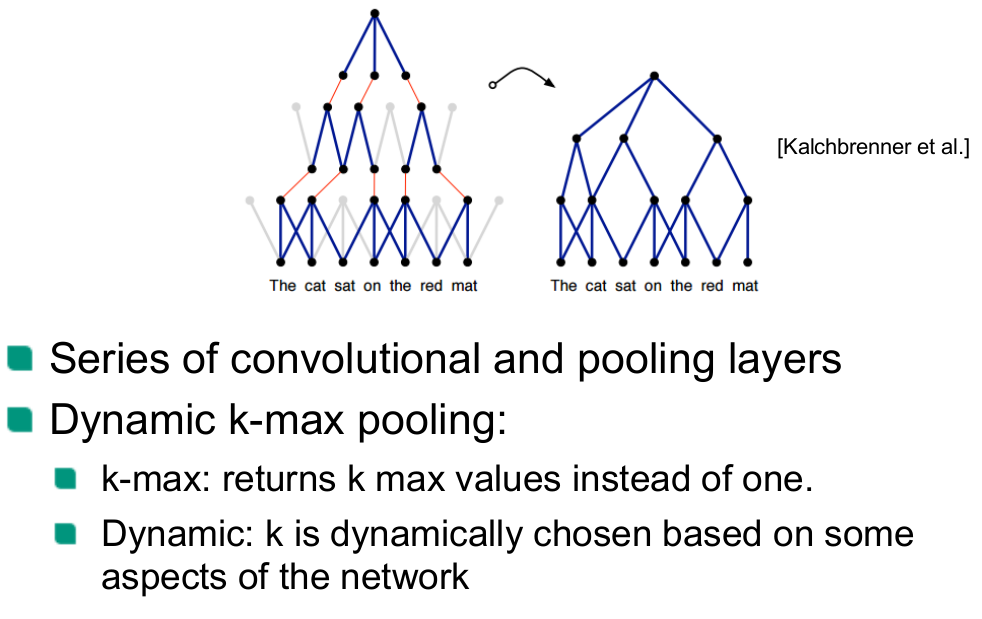
\includegraphics[scale=0.4]{DCNN}
\end{figure}
Advantages
\begin{itemize}
\item A filter is a linguistic feature detector of a class of n-grams
\item Features are extracted independently from their positions.
\item Higher filters can capture syntactic and semantic info.
\end{itemize}
Dynamic k-max pooling:
\[
k_I = max(k_{top}, \lceil \frac{L - I}{L} S \rceil)
\]
$k_{top}$: fixed $k_{top}$ pooling layer on top\\
$I, L$: convolutional layer $I$ over total $L$ convolutional layers where the $k^{th}$ applied on.\\
Properties:
\begin{itemize}
\item Sensitivity to word and n-gram order
\item Have the ability to induce feature graph
\end{itemize}
\newpage
\section{Gradient Optimizations and 2nd order Methods}
\label{sect:gradient-optimization-and-2nd-order-methods}
Idea: Start from a point close to the wanted solution and iteratively move to the point that makes the gradient of the function approache zero (hence \textit{decent}). All weights are initialised with small random numbers.\\
\textbf{Important:} update the parameters in the \textbf{opposite} direction of the gradient:
\[
\mathbf{w} = \mathbf{w} - \eta \mathbf{\nabla}_{\mathbf{w}} L(\mathbf{x}, \mathbf{w})
\]

\subsection{Logistic Regression}
\label{ssect:logistic-regression}
\[
L(\mathbf{x}, \mathbf{w}) = - \sum_k [t_k^x \log(o_k^x) + (1-t_k^x) \log(1-o_k^x)]
\]

\[
o_k^x = \sigma(\mathbf{w} \mathbf{x}_k) = \frac{1}{1 + e^{-\mathbf{w}\mathbf{x}_k}}
\]

\begin{align*}
\nabla_{\mathbf{w}} L &= \frac{\partial L}{\partial \mathbf{o}} \frac{\partial \mathbf{o}}{\partial \mathbf{\sigma}} \frac{\partial \mathbf{\sigma}}{\partial \mathbf{w}} \\
&= (\mathbf{o} - \mathbf{t}) \mathbf{x}
\end{align*}
Update rule:
\[
\mathbf{w} = \mathbf{w} - \eta(\mathbf{o} - \mathbf{t}) \mathbf{x}
\]

\subsubsection{Gradient Descent - General Approach}
\label{sssect:gradient-descent}
\begin{itemize}
	\item init $\mathbf{w}$, chose learning rate $\eta$
	\item iterate:
		\begin{itemize}
			\item grad = $\mathbf{0}$
			\item iterate for every instance of the training data $x \in X$:
				\begin{itemize}
					\item compute output $o_x = \sigma (\mathbf{w} \mathbf{x})$
					\item compute error $E = t_x - o_x$
					\item $grad = grad + E \mathbf{x}$
				\end{itemize}
			\item update $\mathbf{w} = \mathbf{w} + \eta grad$
		\end{itemize}
	\item until a convergence condition is reached (small error or all epochs done)
\end{itemize}

\subsubsection{Batch Gradient Descent}
\label{sssect:batch-gradient-descent}
Works like the normal gradient descent but the weights are updated every \textbf{epoch}!
\begin{itemize}
	\item - iterate whole dataset to perform one update
	\item - slow and memory-intensive
	\item - can not be used for \textit{online} training
\end{itemize}

\subsubsection{Stochastic Gradient Descent}
\label{sssect:stochastic-gradient-descent}
Update the weights right after we have seen \textit{one training instance}. Before each epoch \textit{shuffle} the training set!
\begin{itemize}
	\item + converges much faster
	\item + no huge reuqiremen of memory
	\item + can be used for online training
	\item - approximation of the gradient
	\item - high variance in updating
\end{itemize}

\subsubsection{Mini-Batch Gradient Descent}
\label{sssect:mini-batch-gradient-descent}
Compromise between Batch and Stochastic Gradient descent. Perform one weight update after $k$ training instances (called 1 \textbf{iteration}).
\begin{itemize}
	\item + faster than batch gradient descent
	\item + overcome memory intensity (depends on k)
	\item + can be used for online training
	\item + Faster and more stable than Stochastic Gradient Descent
	\item + fewer smaller weight updates
	\item very easy to parallelze
\end{itemize}

\subsection{Learning Rate Scheduling}
\label{ssect:learning-rate-scheduling}
Decay learning rates, making it smaller as the training is going. From time step $t_d$ (the $t_d^{th} iteration)$, calculate: $\eta_{t+1} = \beta \eta_t$. Choosing learning rates and learning rate scheduling can be tricky.

\subsubsection{Adagrad - ADAptive GRADient method}
\label{sssect:adagrad-apaptive-gradient-method}
\[
\mathbf{w}_t = \mathbf{w}_{t - 1} - \frac{\eta}{\sqrt{G_T + \epsilon}} \nabla_{\mathbf{w}} L(\mathbf{x}, \mathbf{w}_{t-1})
\]
$G_t \in \mathbb{R}^{d \times d}$: diagonal matrix, each diagonal entry is the sum of the squares of the gradients with respect to $w_i$ up to time step t\\
$\epsilon$: small smoothing term that avoids division by zero
\begin{itemize}
	\item + good for sparse data
	\item + no manual tuning of the learning rate (normally $\eta = 0.01$, $\epsilon = 1e^{-8}$)
	\item - have to store $G_t$
	\item - $G_t$ is accumulated $\Rightarrow$ adaptive learning rate is smaller over time
\end{itemize}
\subsubsection{Adadelta}
\label{sssect:adadelta}
Same as Adagrad but only stores a limited history of the gradients (normally 2). 
\begin{align*}
\mathbf{w}_t &= \mathbf{w}_{t - 1} - \frac{RMS[\Delta w]_{t - 1}}{RMS[g]_t} g_t \\
g_t &= \nabla_{\mathbf{w}} L(\mathbf{x}, \mathbf{w}_{t-1}) \\
RMS[\Delta w]_t &= \sqrt{E[\Delta w^2]_t + \epsilon} \\
E[\Delta w^2]_t &= \gamma E[\Delta w^2]_{t-1} + (1 - \gamma) \Delta w_t^2
\end{align*}
- das $E[\Delta w^2]_t$???
\begin{itemize}
	\item + not memory intensiv
	\item + no picking of the learning rate needed
\end{itemize}
\subsubsection{RMSprop}
\label{sssect:rmsprop}
\begin{align*}
\mathbf{w}_t &= \mathbf{w}_{t - 1} - \frac{\eta}{\sqrt{E[g^2]_t + \epsilon}} g_t \\
E[g^2]_t &= \gamma E[g^2]_{t - 1} + g_t^2
\end{align*}
\subsubsection{Adam - ADAptive Moment estimation}
\label{sssect:adam}
\begin{align*}
\mathbf{w}_t &= \mathbf{w}_{t - 1} - \frac{\eta}{\sqrt{\widehat{\mathbf{v}}_t + \epsilon}} \widehat{\mathbf{m}}_t \\
\widehat{\mathbf{m}}_t &= \frac{m_t}{1-\beta_1^t}\\
\widehat{\mathbf{v}}_t &= \frac{v_t}{1-\beta_2^t}\\
m_t &= \beta_1 m_{t - 1} + (1 - \beta_1)g_t \\
v_t &= \beta_2 v_{t - 1} + (1 - \beta_2) g_t^2
\end{align*}
-beta1, beta2??
\begin{itemize}
	\item + faster convergence
	\item - pratically more overfitting
	\item - needs resetting
	\item - needs to store to matrices of past gradients
\end{itemize}
\newpage
% Error Functions
Mean Square Error
Cross Entropy
Classification Figure of Merit
% TODO: Ableitungen und Schaubilder einfügen
\section{Activation Functions}
\label{sect:activation-functions}
The activation functions should have the following properties:
\begin{itemize}
	\item continous
	\item bounded
	\item monotonically increasing
	\item differentiable
\end{itemize}
\subsection{Step Function}
\label{ssect:linear-function}
\[
\varphi(x) = \begin{cases}
1 \: \text{if} x > 0 \\
0 \: \text{if} x \leq 0 \\
\end{cases}
\]
Derivative is always 0
\subsection{Linear Function}
\label{ssect:linear-function}
\[
\varphi(x) = x
\]
Linear functins alone can only solve linear separable problems but can be used in a combination node for function approximation problems.
\subsection{Logistic / Sigmoid Function}
\label{ssect:logistic-function}
\begin{align*}
\varphi(x) = sigmoid(x) &= \frac{1}{1 + e^{-x}} \\
\frac{\delta \varphi(x)}{\varphi(x)} &= \varphi(x) (1 - \varphi(x))
\end{align*}
Good for internal nodes, bad for outpur nodes.
\begin{figure}[h]
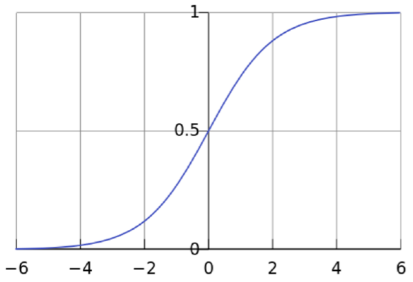
\includegraphics[scale=0.4]{sigmoid}
\end{figure}

\subsection{Hyperbolic Tangent function}
\label{ssect:hyperbolic-tangent-function}
\begin{align*}
\sigma(x) = \tanh(x) &= \frac{e^x - e^{-x}}{e^x + e^{-x}} \\
\frac{\delta \sigma(x)}{\sigma(x)} = 1 - \tanh^2(x) &= 1 - \frac{(e^x - e^{-x})^2}{(e^x + e^{-x})^2}
\end{align*}
\begin{figure}[h]
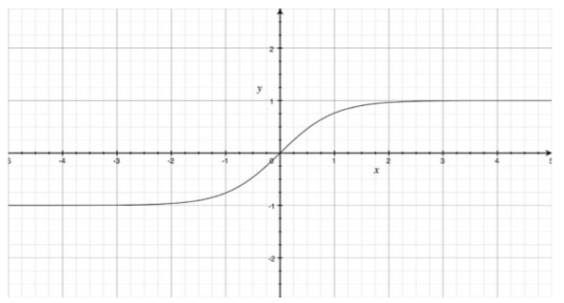
\includegraphics[scale=0.6]{tanh}
\end{figure}
If the input has a mean of 0 then so will the output

\subsection{Softmax Function}
\label{ssect:softmax-function}
\begin{align*}
\varphi(x_j) &= \frac{e^{x_j}}{\sum_k e^{x_k}} \\
\frac{\delta \varphi(x_j)}{\varphi(x_j)} = \varphi(x_j) - \varphi(x_j)^2 &= \varphi(x_j)(1 - \varphi(x_j))
\end{align*}
Outputs an a posteriori probability $p(c | x)$ and is good for classification tasks.

\subsection{Rectified Linear Unit}
\label{ssect:softmax-function}
\begin{align*}
s
\end{align*}
\newpage
% \section{Algorithmen}
\label{sect:algorithmen}

clustering algorithmen
	k-means
	
distanzmaß
	squared error
	Itakura, Saito and Chaffee


% create list of figures etc. 
% caption all graphics and refer to them correctly

% Output eines MLP kann statistisch interpretiert werden: P(W|A), jedoch gilt beim akustichem Modell P(A|W)! -> Überführung: Bayes regel umformulieren. Unterer Teil vom Bruch konstant. P(W): Vorkommnise eines Phonems zählen.

% TODO lvq
% fragen:
% kullback leibner vs cross entropy
% regression
% MSE: legt focus auf die distanz zwischen samples
% levenstein - wort bzw duchstaben abstand
% CFM, MMIE
% cross validation: random oder abschnitte -> die unterteilung der daten in training, test(für mehr info/analysis), validation: und diese werden durchgewechselt
% LSTM mit Backpropagation - input / forget / output
% why fully connected upper layers? -> combine lower level features
\end{document}
